% Rules for the HuroCup Lift and Carry Competition
% Jacky Baltes <jacky@cs.umanitoba.ca> 

\documentclass[12pt]{hurocup}

\begin{document}

\title{\HuroCup: Lift and Carry\\
  Laws of the Game 2009}

\author{Jacky Baltes\\
Autonomous Agents Laboratory\\
University of Manitoba\\
Winnipeg, Manitoba\\
Canada, R3T 2N2\\
Email: jacky@cs.umanitoba.ca\\
WWW: http://www.cs.umanitoba.ca/\~{ }jacky\\[5mm]
Kuo-Yang Tu\\
National Kaohsiung First University of Science and Technology\\
Kaohsiung City, R. O. C.\\
Email: tuky@ccms.nkfust.edu.tw\\
}

\maketitle

\begin{center}
 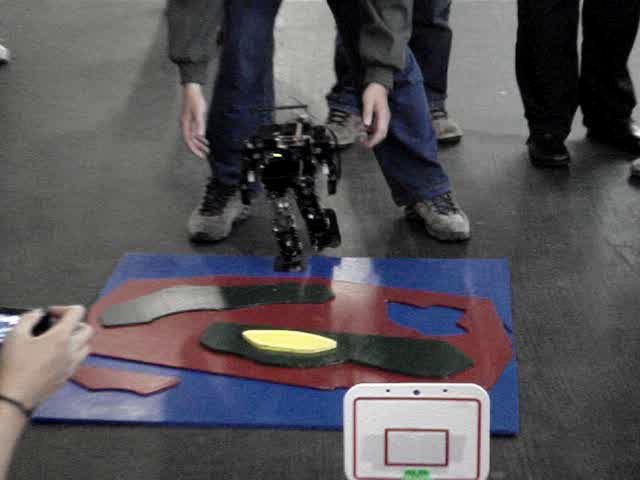
\includegraphics[width=0.7\linewidth]{Figures/lift-and-carry-life}
\end{center}

\begin{abstract}
The following rules and regulations govern the Lift and Carry event in
\HuroCup, a robotic game and robotics benchmark problem for humanoid
robots.
%
\end{abstract}

\section*{Latest Version of the Rules for \HuroCup}
\label{sec:updates}

The latest official version of the rules of the game for \HuroCup\ is
always available from the FIRA \HuroCup\ website (http://www.fira.net).

\newpage

\section{Lift and Carry}
\label{sec:lift-and-carry} 

The goal of this competition is to provide an event that requires
robots to use active balancing. The robots will be fitted with a small
basket. The robots repeatedly walk across an uneven terrain from one
side to the other. Once the robot reaches the end of the uneven
terrain, the referee adds small heavy obstacles into the basket. The
robot must compensate for the extra weight and continue to cross the
uneven terrain.  to walk. The robot that can carry the most weight is
declared the winner of the event.

\section{Laws of the Game: Lift and Carry Competition}
\label{sec:rules-lift-carry}

The following laws describe the specifics of the lift and carry
event. For general specifications relevant to all \HuroCup\ events
(e.g., robot dimensions, playing field and lighting, responsibility of
the referees) please refer to the general \HuroCup\ laws.

\law[LC]{The Field of Play}
\label{lc-field}

\begin{lawlist}[LC]

\item The dimensions of the playing field are at least 180cm by
  180cm.

\item An approximately 1.00m by 1.00m wide uneven terrain is placed by
the referee in the playing field (See
Fig.~\ref{fig:lift-and-carry-field}.

  \begin{figure}
    \begin{center}
      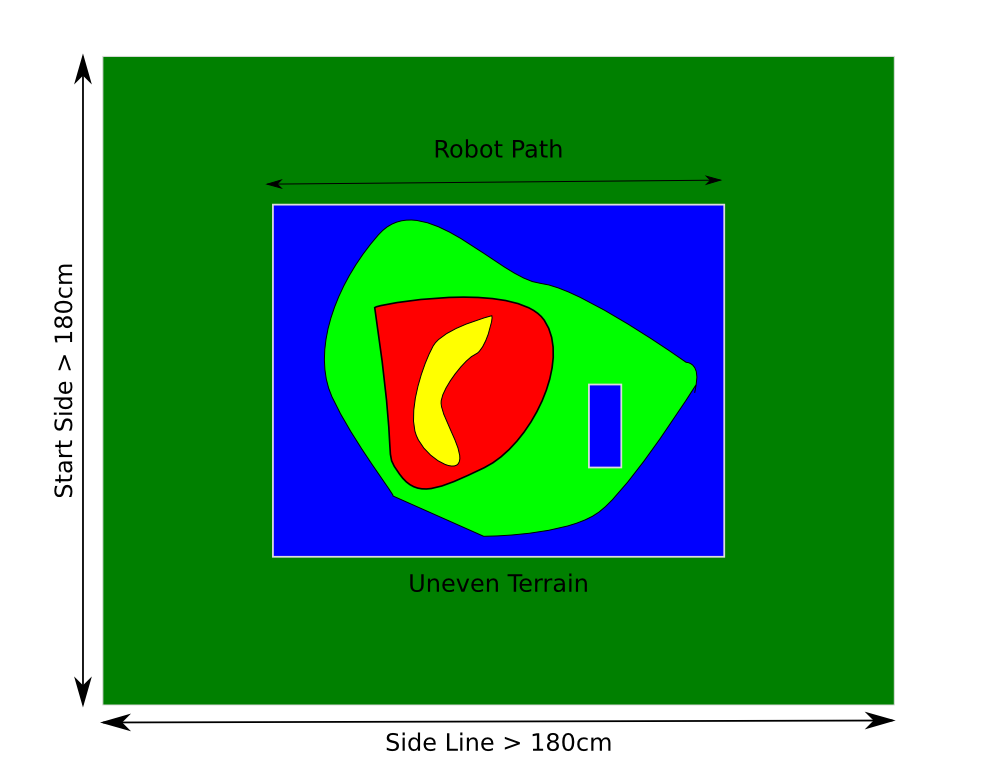
\includegraphics[width=0.7\textwidth]{Figures/lift-and-carry}
    \end{center}
    \caption{The field of play for the lift and carry competition. The
      task for the robot is to cross the uneven terrain repeatedly with
      increasing load.}
    \label{fig:lift-and-carry-field}
  \end{figure}

\item The uneven terrain consists of sheets of hard material such as
corrugated plastic, corrugated cardboard, or wood. 

\item The thickness of a single sheet is between 5mm to 10mm.

\item The uneven terrain is constructed by placing random cut-outs of
the sheets on top of each other. The cut-outs may contain holes.  The
exact shape of the uneven terrain is determined by the local
organizing chair.

\item The sheets are colour coded, that is sheets at different heights
have different colours as shown in Fig.~\ref{fig:uneven-terrain}.

  \begin{figure}
    \begin{center}
      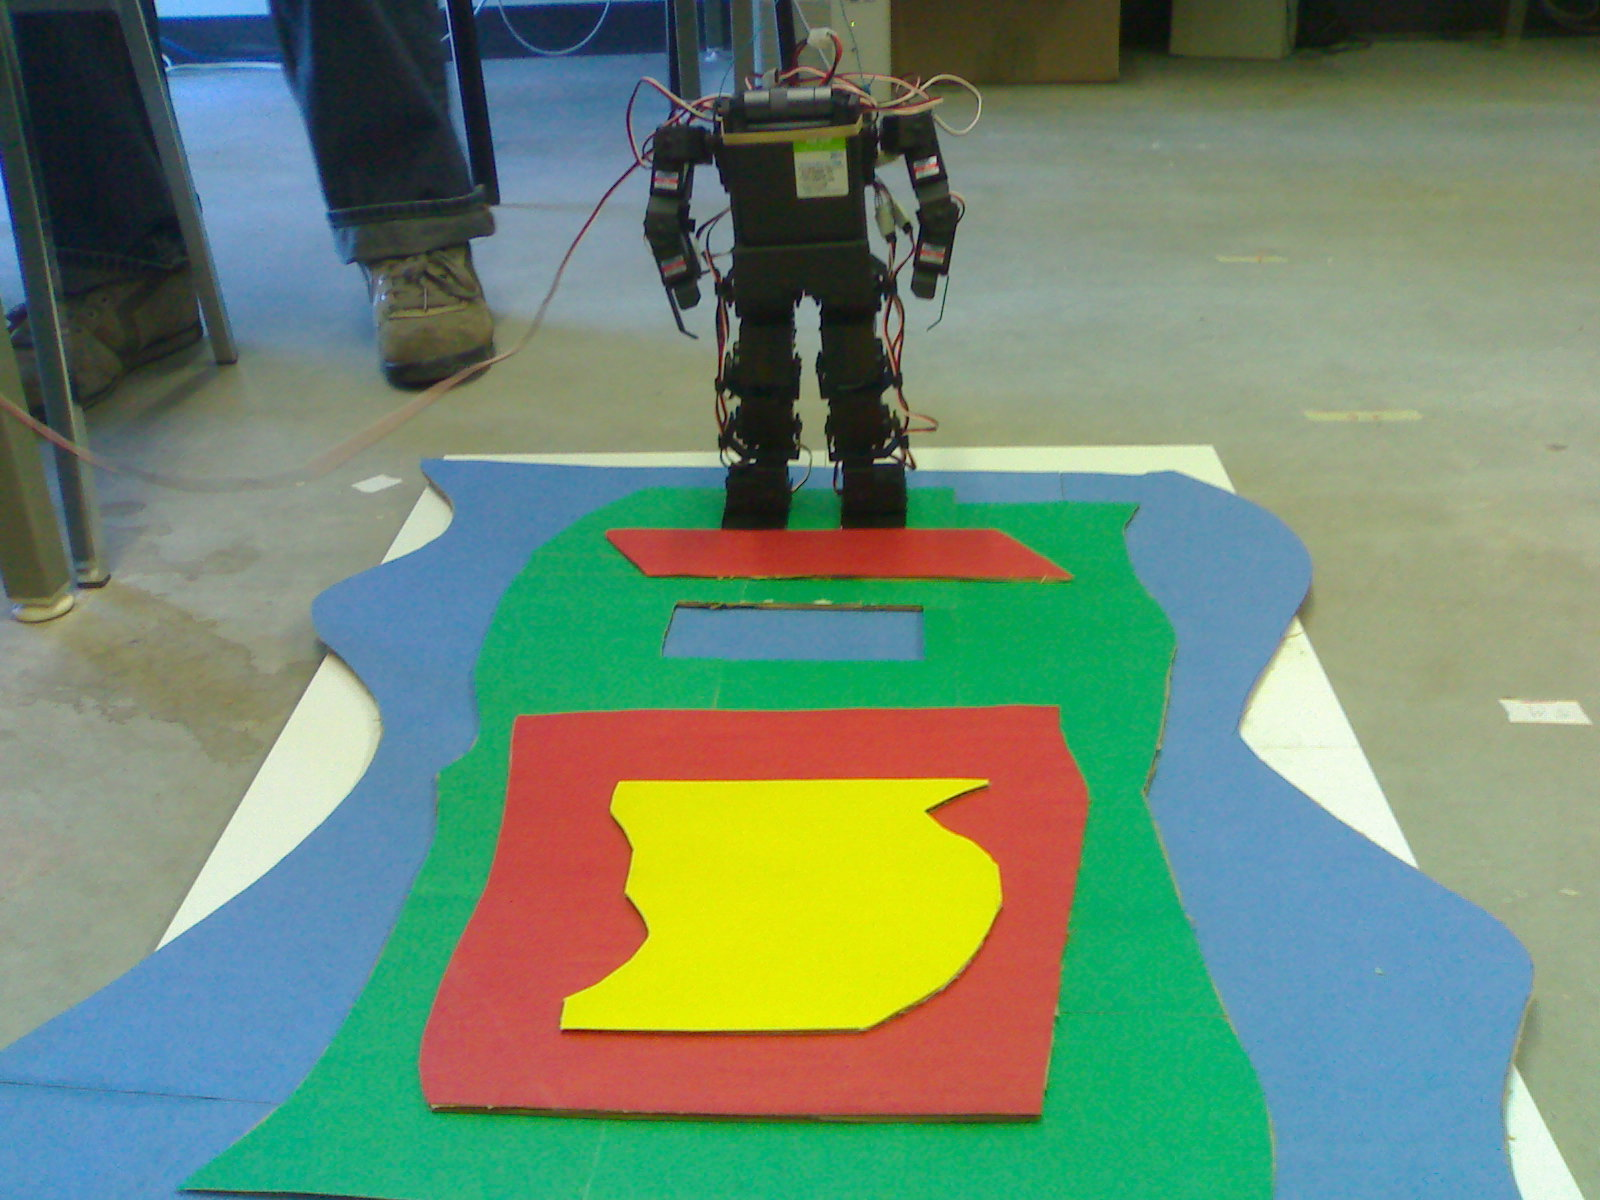
\includegraphics[width=0.8\textwidth]{Figures/uneven-terrain}
    \end{center}
    \caption{A sample uneven terrain}
    \label{fig:uneven-terrain}
  \end{figure}

\item Teams may place small coloured markers in the goal are as long
  as they do not interfere with other teams.

\end{lawlist}

\law[LC]{Number of Robots}

\begin{lawlist}[LC]
\item A single robot competes in a match.
\end{lawlist}

\law[LC]{The Players}

Please refer to the general \HuroCup\ laws for a description of
the players.

\law[LC]{The Referee}

Please refer to the general \HuroCup\ laws for a description of
the referee.

\law[LC]{The Assistant Referee}

Please refer to the general \HuroCup\ laws for a description of
the assitant referee.

\law[LC]{Game Play}

\begin{lawlist}[LC]

\item A single robot is designated the runner. All other robots
  must be outside of the playing field.

\item The only robot allowed to move during a run is the
  designated runner.

\item The runner must be fitted with a small basket or bucket (see
  Fig.~\ref{fig:robot-lift-and-carry-basket} for an example), which is
  able to hold as many batteries as the team wants the robot to carry.

  \begin{figure}
    \begin{center}
      \begin{tabular}{cc}
        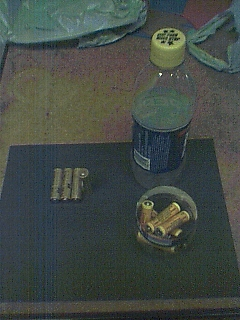
\includegraphics[width=0.40\linewidth]{Figures/robot-lift-and-carry-basket}
        &
        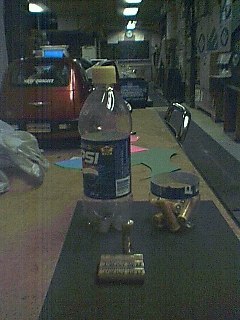
\includegraphics[width=0.40\linewidth]{Figures/robot-lift-and-carry-basket2}
        \\
      \end{tabular}
    \end{center}
    \caption{A suitable basket for the lift and carry challenge on the
      right and suitable weights (Standard AA batteries) in front.
      Such a basket must be fitted to the robot before the lift and
      carry challenge. A standard 591ml soft drink bottle is shown for
      comparison. The basket in the picture was constructed by cutting
      the bottom off the soft drink bottle.}
    \label{fig:robot-lift-and-carry-basket}
  \end{figure}

\item The runner will be placed at one end of the uneven terrain in
the middle of the terrain.

\item At the beginning of the competition, the referee will place one
  weight in the basket attached to the robot.

\item The referee will signal the start of the competition by blowing
  the whistle.

\item After the referee gives the start signal, the robot must cross
  the uneven terrain to reach the other side.

\item A robot is not allowed to leave the uneven terrain along the sides.

\item Each robot may have at most one human handler associated with
  it.

\item \label{lc-handler5} The human handlers are not allowed to
  interfere in any way with other robots, the referee, or other human
  handlers.

\item \label{lc-handler6} A human handler may only enter the playing
  field or touch his/her robot with the permission of the referee.

\item The end of the competition is signaled by the referee by
  blowing the whistle a second time.
  The referee terminates the competition if
  \begin{itemize}
  \item the robot has crossed the uneven terrain with a maximum load,
  \item the robot was unable to cross the uneven terrain within 2 minutes,
  \item the robot falls and is unable to get up on its own or is
    immobilized by a technical defect, 
  \item the robot leaves the uneven terrain along the side lines,
  \item at least one minute has elapsed since the start of the
    competition and it is unlikely in the opinion of the referee that
    the robot will cross the finish line within the remaining time.
  \end{itemize}

\item At the end of the run, another robot will be designated the
  runner.

\end{lawlist}

\law[LC]{Method of Scoring}

\begin{lawlist}[LC]
\item Any robot that has not crossed the uneven terrain at least once is
  automatically awarded $0$ rank.
\item Among the robots that have crossed the uneven terrain at least
  once, the robots are ranked (i.e., 1st place, 2nd place) based on
  the greater number of batteries carried.

\item The point allocation for robots is as follows:
  \begin{itemize}
  \item The first ranked robot is awarded $10$ points.
  \item The second ranked robot is awarded $8$ points.
  \item The third ranked robot is awarded $6$ points.
  \item The fourth, fifth, sixth, and seventh place robots are awarded
    $4$,$3$,$2$, and $1$ point respectively.  A summary of the point
    allocation for placings is shown in table~\ref{point-allocation}.

    \begin{table}
      \begin{center}
        \begin{tabular}{l|l}
          \hline
          Place & Points scored \\
          \hline
          1 (Winner) & 10 \\
          2          & 8 \\
          3          & 6 \\
          4          & 4 \\
          5          & 3 \\
          6          & 2 \\
          7          & 1 \\
          8, 9, ...  & 0 \\
          \hline
        \end{tabular}
      \end{center}
      \caption{Point allocation for placings in the \HuroCup\ events.}
      \label{point-allocation}
    \end{table}
  \end{itemize}

\item In case of a tie between $n$ robots with rank $k$, all robots
 will be awarded rank $k$ and receive the average of the scores for
 ranks $k$ to $k+n$.  For example, if the robots $A,B,C,D$ scored $10,
 8, 8, 4$ goals respectively, then robot $A$ will be declared the
 winner (1st place) and receive 10 points, both robots $B$ and $C$
 will be declared 2nd place finishers and receive $(8+6)/2=7$, and
 robot $D$ will be declared the fourth place finisher and receive $4$
 points.

\end{lawlist}

\begin{decisions}
\item For the 2009 competition, the technical committee decided that
in addition to the restrictions given above, the uneven terrain
includes the following simplifications:
\begin{itemize}
\item The uneven terrain will only contain steps wich move one level
up or down.
\item The minimum distance between edges of the sheets is 5 cm.
\end{itemize}
These additional constraints are targeted at simplifying the lift and
carry competition over uneven terrain.

\end{decisions}

\end{document}


% *** Local Variables: ***
% *** mode: LaTeX ***
% *** mode: outline-minor ***
% *** mode: auto-fill ***
% *** outline-regexp: "% !\\|\\\\\\(sub\\)*section" ***
% *** TeX-command-default: "LaTeX PDF" ***
% *** End: ***
